\setAuthor{Jaan Kalda}
\setRound{lõppvoor}
\setYear{2017}
\setNumber{G 6}
\setDifficulty{5}
\setTopic{Elektriahelad}

\prob{Viisnurk}
Leidke joonisel toodud skeemis ampermeetri ja voltmeetri näidud. Kõik takistid on takistusega $R=\SI{1}{\ohm}$, pinge patarei klemmidel $U=\SI{7}{\volt}$.

\begin{center}
	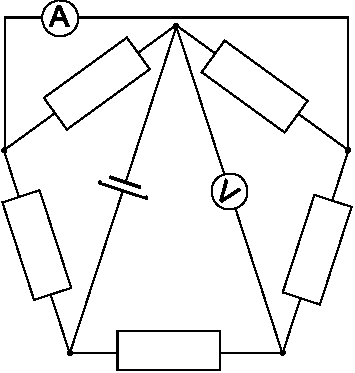
\includegraphics[width=0.4\textwidth]{2017-v3g-06-viisnurk}
\end{center}

\hint
Elektriskeemi käitumisest arusaamiseks tasub skeem selgemalt ümber joonistada, nii et ampermeeter on asendatud juhtmega ja voltmeeter lihtsalt kõrvaldatud.

\solu
Joonistame lihtsustatud skeemi, arvestades et ampermeeter ja voltmeeter 
on ideaalsed. See tähendab, et ampermeetri võib asendada juhtmega ja 
voltmeetri lihtsalt kõrvaldada. Tähistame uue skeemi sõlmpunktid 
tähtedega P --- patarei plussklemm; M --- patarei miinusklemm; A --- 
ampermeetri asukoht; V --- voltmeetri alumine klemm. Takistid tähistame 
numbritega ühest viieni, liikudes päripäeva ja alustades viisnurga 
ülemisest tipust paremale jäävast takistist. Tulemus on toodud joonisel 
oleval skeemil.
\begin{center}
	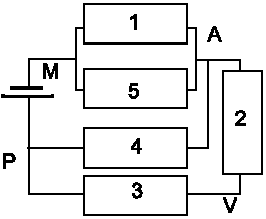
\includegraphics[width=0.5\textwidth]{2017-v3g-06-viisnurk-lah}
\end{center}
Kirchoffi vooluseaduse tõttu on ampermeetri vool võrdne 
takistite 4 ja 5 voolude vahega, sest see osa voolust, mis läks läbi takisti 4, aga ei läinud läbi takisti 5, pidi järelikult läbi ampermeetri minema. Voltmeetri näit on võrdne klemmide 
M ja V vahelise pingega.
Skeemis on takistid 1 ja 5 paralleelselt, seega on nende takistus kokku $\frac{1}{2}\si{\ohm}$. Takisti 4 on paralleelselt 
takistite 2 ja 3 jadaühendusega, seega on nende takistus
\[
\frac{1}{\frac{1}{1\si{\ohm}}+\frac{1}{2\si{\ohm}}} = \frac 23 \si{\ohm}.
\]
Terve skeemi kogutakistus on seega
\[
R_K=\left(\frac 12 + 
\frac 23\right)\si{\ohm}=\frac 76\si{\ohm},
\]
koguvool seega $I=\mathcal 
E/R_K=\SI{6}A$. Takistitest 1 ja 5 läheb sama palju voolu läbi,
mistõttu takisti 5 vool on $I_5=\frac 12 I=\SI{3}A$ ja pingelang sellel takistil on \SI{3}{\volt}. Seega on punktide A ja P vahel pinge \SI{4}{\volt} ja vool läbi takisti 4 
on $I_4=\frac{\SI{4}{\volt}}{\SI{1}{\ohm}}=\SI{4}A$. Ampermeetri
näit on seega $I_4-I_5=\SI 1A$.

Pinge M ja V vahel on patarei pingest väiksem takisti 3 pinge võrra. Kuna punktide A ja P vahel oli pinge \SI{4}{\volt}, siis arvestades, et takistid 2 ja 3 on samasugused ning jadamisi ühendatud, on takistil 3 pinge \SI{2}V. 
See annab voltmeetri pingeks $\SI{7}V -\SI{2}V= \SI{5}V$.

\probeng{Pentagon}
Find the readings of the ammeter and the voltmeter in the circuit diagram given in the drawing. All the resistors have a resistance $R=\SI{1}{\ohm}$, voltage on the battery’s leads is $U=\SI{7}{\volt}$. 
\begin{center}
	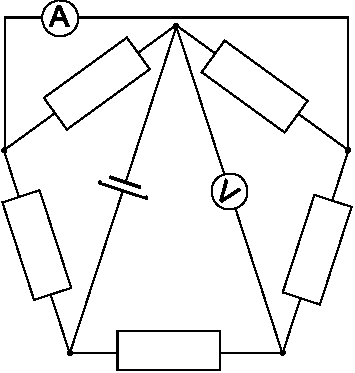
\includegraphics[width=0.4\textwidth]{2017-v3g-06-viisnurk}
\end{center}

\hinteng
To understand the circuit a clearer and simpler version of it should be sketched so that the ammeter is replaced by a wire and the voltmeter is just removed.

\solueng
Let us draw a simplified diagram while considering that the ammeter and voltmeter are ideal. This means that the ammeter can be replaced by a wire and the voltmeter can just be removed. Let us mark the nodes of the new diagram as the letters P – battery’s minus lead; M- battery’s plus lead; A – the location of the ammeter; V – the bottom lead of the voltmeter. We mark the resistors with numbers from one to five, moving clock-wise and beginning from the resistor that is to the right of the pentagon’s upper tip. In result we get the diagram in the figure.
\begin{center}
	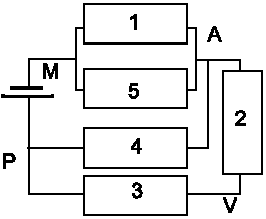
\includegraphics[width=0.5\textwidth]{2017-v3g-06-viisnurk-lah}
\end{center}
Due to the Kirchhoff’s current law the ammeter’s current is equal to the current difference of resistors 4 and 5. This is because the part of the current that went through the resistor 4 but not through the resistor 5 had to therefore go through the ammeter. The reading of the voltmeter is equal to the voltage between the leads M and V. The resistors 1 and 5 are parallel in the diagram so their total resistance is $\frac{1}{2}\si{\ohm}$. The resistor 4 is parallel to the series connection of resistors 2 and 3, therefore their resistance is
$$\frac{1}{\frac{1}{1\si{\ohm}}+\frac{1}{2\si{\ohm}}} = \frac 23 \si{\ohm}. $$ 
The total resistance of the whole diagram is therefore $R_K=\left(\frac 12 + 
\frac 23\right)\si{\ohm}=\frac 76\si{\ohm}$, the total current $I=\mathcal 
E/R_K=\SI{6}A$. The same amount of current goes through the resistors 1 and 5 which is why the current of resistor 5 is $I_5=\frac 12 I=\SI{3}A$ and its voltage drop is 3 V. Thus, the voltage between the points A and P is 4 V and the current that goes through the resistor 4 is $I_4=\frac{\SI{4}{\volt}}{\SI{1}{\ohm}}=\SI{4}A$. The reading of the ammeter is therefore $I_4-I_5=\SI 1A$.\\
The voltage between M and V is smaller from the voltage of the battery by the voltage of the resistor 3. Because the voltage between the points A and P was 4 V and considering that the resistors 2 and 3 are identical and connected in series then the voltage on the resistor 3 is 2 V. This means that the voltage on the voltmeter is $\SI{7}V -\SI{2}V= \SI{5}V$.
\probend